% !TEX TS-program = pdflatex
% !TEX encoding = UTF-8 Unicode

\documentclass[letterpaper, 11pt]{article}


% layout/spacing related packages
\usepackage[margin=1in]{geometry}
\usepackage{setspace}\onehalfspace
\usepackage{microtype}


% Math related packages
\usepackage{amsmath} \allowdisplaybreaks
\usepackage{amssymb}
\usepackage{amsthm}
%\theoremstyle{definition}    % if you want normal upright font styles for theorems.
\newtheorem{theorem}{Theorem}
\newtheorem{lemma}{Lemma}
\newtheorem{assumption}{Assumption}
\newtheorem{proposition}{Proposition}
\newtheorem{definition}{Definition}


% bibliography and reference related packcages
\usepackage{natbib}
\usepackage{bibentry}


\usepackage{booktabs} % for toprule, midrule, bottomrule
\usepackage{graphicx}
\usepackage{appendix}
\usepackage[counterclockwise]{rotating} % for sidewaystable
\usepackage{subcaption} % for subfigure
\usepackage[normalem]{ulem} % for uline
\usepackage{showexpl}
\usepackage{threeparttable} % for tables with footnotes

\usepackage[hyphens]{url}
\usepackage[bookmarks=false,hidelinks]{hyperref}

\usepackage{tikz}
\usetikzlibrary{automata,calc,trees,positioning,arrows,chains,shapes.geometric,%
decorations.pathreplacing,decorations.pathmorphing,shapes,%
matrix,shapes.symbols,plotmarks,decorations.markings,shadows}

\usepackage{pgf}
\pgfdeclarelayer{background}
\pgfdeclarelayer{foreground}
\pgfsetlayers{background,main,foreground}


\usepackage{authblk}
\renewcommand\Authfont{\sf\Large}
\renewcommand\Affilfont{\rm\small}





%%%%%%%%%%%%%% MACRO %%%%%%%%%%%%%%%%%%%%%%%%%%%%%%%%%%%%%%
\newcommand{\email}[1]{{\href{mailto:#1}{\nolinkurl{#1}}}}

\usepackage{bm}
\renewcommand{\vec}[1]{\bm{#1}}
\newcommand{\mat}[1]{\bm{#1}}
\newcommand{\set}[1]{\mathcal{#1}}

% https://tex.stackexchange.com/questions/265689/ignore-greek-letters-using-mathcal
\DeclareMathSymbol{\Gamma}{\mathord}{operators}{"00}
\DeclareMathSymbol{\Delta}{\mathord}{operators}{"01}
\DeclareMathSymbol{\Theta}{\mathord}{operators}{"02}
\DeclareMathSymbol{\Lambda}{\mathord}{operators}{"03}
\DeclareMathSymbol{\Xi}{\mathord}{operators}{"04}
\DeclareMathSymbol{\Pi}{\mathord}{operators}{"05}
\DeclareMathSymbol{\Sigma}{\mathord}{operators}{"06}
\DeclareMathSymbol{\Upsilon}{\mathord}{operators}{"07}
\DeclareMathSymbol{\Phi}{\mathord}{operators}{"08}
\DeclareMathSymbol{\Psi}{\mathord}{operators}{"09}
\DeclareMathSymbol{\Omega}{\mathord}{operators}{"0A}

\newcommand{\LB}{\mathsf{LB}}
\newcommand{\UB}{\mathsf{UB}}		

\usepackage{xcolor}
\newcommand{\note}[1]{{\Large\bf#1}}
\newcommand{\bluenote}[1]{{\Large\color{blue}#1}}
\newcommand{\rednote}[1]{{\Large\color{red}#1}}

\usepackage{etoolbox}
% To use, for example, \Ac for \mathcal{A}.  Requires "etoolbox" package
\makeatletter
\def\do#1{\@namedef{#1c}{\ensuremath{\mathcal{#1}}}}
\docsvlist{A,B,C,D,E,F,G,H,I,J,K,L,M,N,O,P,Q,R,S,T,U,V,W,X,Y,Z}
\makeatother

\def\Eb{\mathbb{E}}
\def\Rb{\mathbb{R}}
%\def\response{[$\Longrightarrow$]}

\newenvironment{response}
{ [$\Longrightarrow$]\sf }
{ \hfill \rule{1ex}{1ex} }

\newcommand{\dx}{\mathop{}\!\mathrm{d}x}
\newcommand{\dy}{\mathop{}\!\mathrm{d}y}
\newcommand{\dz}{\mathop{}\!\mathrm{d}z}
\newcommand{\dt}{\mathop{}\!\mathrm{d}t}

\renewcommand{\bar}[1]{\mkern 1.5mu\overline{\mkern-1.5mu#1\mkern-1.5mu}\mkern 1.5mu}



%%%%%%%%%%%%%%%%%%%%%%%%%%%%%%%%%%%%%%%%%%%%%%%%%%%%%%%%
% To show LaTeX code examples

\usepackage{fancyvrb,listings}
\lstset{
   breaklines=true,
   basicstyle=\linespread{0.8}\ttfamily\scriptsize,
   aboveskip=0pt,
   belowskip=0pt
}
\newenvironment{example}
 {\VerbatimOut{\jobname.tmp}}
 {\endVerbatimOut
 \begin{center}
 \fbox{
	 \begin{minipage}[c]{0.48\textwidth}
	  \lstinputlisting{\jobname.tmp}
	 \end{minipage}
   }
 \fbox{
 	\begin{minipage}[c]{0.38\textwidth}
 	 \scriptsize
	 \input{\jobname.tmp}
  	\end{minipage}
  }
  \end{center}
 }

%%%%%%%%%%%%%%%%%%%%%%%%%%%%%%%%%%%%%%%%%%%%%%%%%%%%%%%%





\title{A LaTeX Template for Writing Papers}
\author[1]{First Author}
\author[2]{Second Author}
\author[3]{Changhyun Kwon\footnote{Corresponding Author: \email{chkwon@usf.edu}}}
\affil[1]{Department of First Engineering, First University}
\affil[2]{Department of Second Engineering, First University}
\affil[3]{Department of Industrial and Management Systems Engineering, University of South Florida}

\date{\today}

%\usepackage{showlabels}
%\usepackage[final]{showlabels}


\begin{document}
\maketitle

\begin{abstract}
This document provides some useful tips as well as serve a template for writing a paper in LaTeX.
To understand how LaTeX works, you should compare the source code and the output PDF.\\
\noindent\textbf{Keywords:} keyword1; keyword2; keyword3
\end{abstract}


%\rednote{You need to open \texttt{template.tex} file and read it. Compare \texttt{.tex} file with the output \texttt{.pdf} file as you read \texttt{.tex} file.}

\rednote{When you read this PDF file, please also read .tex file together.}

\bluenote{This document contains several custom commands and packages preferred by Dr. Kwon.
Graduate students of Dr. Kwon are encouraged to follow his tastes.}


\section{Editor} \label{sec:editor}

For most people, I recommend TeXworks (a text editor) for editing .tex files and JabRef (a reference management tool) for editing .bib files.
Mac users can also use TeXShop and BibDesk, alternatively.
TeXworks comes with your LaTeX distribution (TeXLive recommended).
You can download/install JabRef for free.

TeXworks has a built-in PDF viewer.
The best part of TeXworks is forward/backward PDF sync.
After compiling your .tex file, do `Ctrl + Click' or `Command + Click' on some text part in the .tex file.
It will send you to the corresponding part in the output PDF file.
While reading your PDF file (in TeXworks), also do `Ctrl + Click' or `Command + Click' on some text part in the .pdf file.
It will again send you to the corresponding part in the source TeX file.
Use this functionality to read this document.











\section{Text} \label{sec:paragraph}
In LaTeX, just enter an empty line for a new paragraph.

Like this. blah blah blah blah blah blah blah blah blah blah blah blah blah blah blah blah blah blah blah blah blah blah blah blah blah blah blah blah blah blah blah blah blah blah blah blah blah blah blah blah blah blah blah blah blah blah blah blah.

And like this.
Ob-la-di ob-la-da.
Ob-la-di ob-la-da.
Ob-la-di ob-la-da.
Ob-la-di ob-la-da.
Ob-la-di ob-la-da.
Ob-la-di ob-la-da.
Ob-la-di ob-la-da.
Ob-la-di ob-la-da.
Ob-la-di ob-la-da.
Ob-la-di ob-la-da.
Ob-la-di ob-la-da.
Ob-la-di ob-la-da.
Ob-la-di ob-la-da.
Ob-la-di ob-la-da.
Ob-la-di ob-la-da.
Ob-la-di ob-la-da.


\subsection{Do not use backslashes}

Don't use double backslashes \verb|\\| for a new paragraph as done in this paragraph.
Double backslashes will be used in tables and equations only.
Some random text here, there, and everywhere.
Some random text here, there, and everywhere.
Some random text here, there, and everywhere.
Some random text here, there, and everywhere.  \\
If you use double backslashes for a new paragraph, it will look very bad.
Some random text here, there, and everywhere.
Some random text here, there, and everywhere.
Some random text here, there, and everywhere.
Some random text here, there, and everywhere.

\subsection{Emphasizing}
If you want to \emph{emphasize} some \emph{words}, use \verb|\emph{...words..}|, instead of \verb|\textit{...words..}|.

\subsection{Quotation marks}

Quotation marks are input differently in LaTeX.
\begin{example}
``Hello World''
"Hello World"

`linear problem'
'linear problem'
\end{example}
The key for \verb|`| is usually located left to the key for number 1.


\subsection{Dashes}

There are different kinds of `-':

\begin{description}
\item [Hyphen] is a single `-' in text mode.
\begin{example}
shortest-path
\end{example}

\item [En dash] is a double `-' in text mode.
\begin{example}
1999--2015,
New York--London flight,
constraints \eqref{const2}--\eqref{const5}
\end{example}

\item [Em dash] is a triple `-' in text mode.
\begin{example}
Since 2007, the consensus of the economic establishment---bankers, policymakers, CEOs, stock analysts, pundits---has been catastrophically wrong.
\end{example}

\item [Minus] is a single `-' in math mode.
\begin{example}
 $-310$, $x-y$
\end{example}
\end{description}
Read more at \url{https://en.wikipedia.org/wiki/Dash}.














\section{Citation and Cross-Referencing} \label{sec:citation}

You need to provide \texttt{.bib} files.
Look at the end of this document for something like `bibliography'.
This template uses \verb|sample_ref.bib|.
Also learn how to use BibTeX. (Google it!)

\begin{itemize}
\item Textual citation:
\begin{example}
\citet{Kwon2013rsp}
\end{example}

\item Parenthetical citation:
\begin{example}
\citep{Kwon2013rsp}
\end{example}

\item Multiple parenthetical citations:

\begin{example}
\citep{Bertsimas2004,Chaerani2005,Kouvelis1996,gabrel2012recent}
\end{example}

\item If you need multiple \emph{textual} citations, it is better to write:
\begin{example}
\citet{Bertsimas2004}, \citet{Chaerani2005}, \citet{Kouvelis1996}, and \citet{gabrel2012recent},
\end{example}

instead of
\begin{example}
\citet{Bertsimas2004,Chaerani2005,Kouvelis1996,gabrel2012recent}.
\end{example}

\end{itemize}

See them in action:
\begin{quote}
When the uncertain set is box-constrained, the RSP problem can be solved in polynomial time \citep{Bertsimas2003network}, while the problem is NP-hard when the uncertain set is an ellipsoid \citep{Bertsimas2004,Chaerani2005} and a set of scenarios \citep{Kouvelis1996}.
We refer readers to \citet{ben2009robust} and \citet{gabrel2012recent} and references therein for general robust optimization methods.
\end{quote}

For cross-referencing, you should \emph{never} do
\begin{example}
Section 1.
\end{example}
You must always do
\begin{example}
Section \ref{sec:editor}.
\end{example}
Find where \verb|\label{sec:editor}| is in this \verb|.tex| document.

If you see ?? in your PDF, you would need to compile your LaTeX code one more time (or, some errors).

Always use cross-referencing:
\begin{example}
Equation \eqref{const1} or (\ref{const1}).
\end{example}

\begin{example}
Table \ref{tbl:bad_example}.
\end{example}

\begin{example}
Figure \ref{fig:map}.
\end{example}















\section{Math} \label{sec:math}

\subsection{Inline equations}

\begin{example}
Inline equations can be like $\sum_{j:(i,j)\in\Ac} x_{ij}$.
\end{example}

\subsection{Single-line equations}

A single line equation:
\begin{example}
\begin{equation}
 \sum_{j:(i,j)\in\Ac} x_{ij} = 1 \quad \forall i\in\Nc \label{const1}
\end{equation}
\end{example}
I used \verb|\Ac| as a shorthand for \verb|\mathcal{A}| to denote $\Ac$.

\subsection{Notation consistency}

Try to give some consistency in your notation.
I usually use calligraphic letters to denote sets like set of nodes $\Nc$, set of arcs $\Ac$, set of shipments $\Sc$ as in $n\in\Nc$ or $\sum_{s\in\Sc} z_s$, and so on.
Lower-case alphabets for variables like $x_{ij}$, $y_i$, and $z_j$.
Upper-case roman alphabets like $N$, $A$, and $S$ for constants as in $n=1,...,N$ or $\sum_{s=1}^S x_s$.
I usually use lower-case Greek letters for dual variables: $\lambda_i$, $\rho_j$, etc.
Upper-case Greek letters may be some special sets or sets of dual variables: $\Lambda$, $\Theta$, etc.


\subsection{Multiple-line equations}

Multiple lines:
\begin{example}
\begin{align}
 a + b & = c \label{const2} \\
 a + b & = c \nonumber \\
 a + b & = c \label{const3} \\
 a + b & = c \label{const4} \\
 a + b & = c \label{const5}
\end{align}
\end{example}
Note \verb|\nonumber| in the second line, and no \verb|\\| in the last line.

\subsection{Single-line equations in multiple lines}

A single equation that stretches to multiple lines
\begin{example}
\begin{multline}
 \sum a_i + \sum b_i \\
 + \sum c_i + \sum d_i \\
 + \sum e_i + \sum f_i \\
 + \sum g_i + \sum h_i = 1
\end{multline}
\end{example}

\subsection{Cross-referencing}

When you want cross-referencing, do this:
\begin{example}
\eqref{const1}, or \eqref{const2}--\eqref{const5}.
\end{example}

\subsection{Equations without numbering}

If you don't want numbering, just add \verb|*|, like:
\begin{example}
\begin{equation*}
 a + b = c
\end{equation*}
\end{example}
or
\begin{example}
\[
  a + b = c
\]
\end{example}
or
\begin{example}
\begin{align*}
 a + b & = c \\
 a + b & = c
\end{align*}
\end{example}


\subsection{Do not use words}
Please do not use words for variables.
\begin{itemize}
\item Don't:
\begin{example}
 $counter_1 = 3 + 10$
\end{example}
where $counter_1$ may be confused with $c \times o \times u \times n \times t \times e \times r_1$.

\item Instead do:
\begin{example}
 $c_i = 3 + 10$
\end{example}
	or
\begin{example}
 $\text{counter}_1 = 3 + 10$
\end{example}
	or
\begin{example}
 $\textsf{counter}_1 = 3 + 10$
\end{example}
depending on the context.
\end{itemize}


\subsection{Vectors and Matrices}
You can use
\begin{example}
$\vec{x}$ as a vector of $x_{ij}$.
\end{example}
Some matrices
\begin{example}
$\mat{A}$ and $\mat{B}$.
\end{example}

Some vectors are here:
\begin{example}
\[
 \vec{y} = \begin{bmatrix}
             3 \\
             2 \\
             1
           \end{bmatrix}
\]
\end{example}
\begin{example}
\[
 \vec{z} = \begin{bmatrix}
              z_1 \\
              z_2 \\
              \vdots \\
              z_n
           \end{bmatrix}
\]
\end{example}


A matrix is here:
\begin{example}
\[
 \mat{A} = \begin{bmatrix}
            a_{11} & \cdots & a_{22}  \\
            \vdots & \ddots & \vdots  \\
            a_{1n} & \cdots & a_{nn}
           \end{bmatrix}
\]
\end{example}
If you like curly brackets:
\begin{example}
\[
 \mat{A} = \begin{pmatrix}
            a_{11} & \cdots & a_{22}  \\
            \vdots & \ddots & \vdots  \\
            a_{1n} & \cdots & a_{nn}
           \end{pmatrix}
\]
\end{example}








\subsection{Theorems}

You can write a theorem with a proof.

\begin{example}
\begin{theorem} \label{thm:fundamental}
If one is not drunken, the following is true:
\begin{equation}
	1 + 2 = c
\end{equation}
where $c$ is a constant that represents 3.
\end{theorem}
\end{example}

\begin{example}
\begin{proof}
Obvious.
\end{proof}
\end{example}

\begin{example}
\begin{definition}[Convexity]
A convex function is defined ...
\end{definition}
\end{example}

\begin{example}
\begin{lemma}[Kwon's Lemma]
Lemma............
\end{lemma}
\end{example}

\begin{example}
\begin{proof}
We can prove this lemma by using Theorem \ref{thm:fundamental}.
\end{proof}
\end{example}












\section{Tables}


\begin{table} \centering
\caption{The table caption is above the table. Text to the left, numbers to the right. }
\label{tbl:example}
\begin{tabular}{l l r r}
\toprule
Name		& Location		&  Number	& Number \\
\midrule
Michael		& Chicago			&      10   &   3.190  \\
Sara		& Montreal			&     110   & 123.148  \\
Sandra		& LA				&    1210   &   3.000  \\
Alexander	& San Francisco		&       8   &   0.000  \\
\bottomrule
\end{tabular}
\end{table}

\begin{table} \centering
\caption{A bad presentation.}
\label{tbl:bad_example}
\begin{tabular}{c c l l}
\toprule
Name		& Location		&  Number	& Number \\
\midrule
Michael		& Chicago			&      10   &   3.190  \\
Sara		& Montreal			&     110   & 123.148  \\
Sandra		& LA				&    1210   &   3.000  \\
Alexander	& San Francisco		&       8   &   0.000  \\
\bottomrule
\end{tabular}
\end{table}

When you prepare tables, please just ignore the positioning of tables in the final PDF file.
I put the code for Table \ref{tbl:example} above this text and the code for Table \ref{table:8-node} below this text.
Their actual locations in the output PDF file will be determined by LaTeX. Table \ref{tbl:bad_example} is a bad presentation of Table \ref{tbl:example}.
Tables \ref{tbl:example}--\ref{table:8-node} are small tables.
If you have a big table like Table \ref{table:EDOandLINGO}, then you can use `\texttt{sidewaystable}'.
However, it is best to redesign the table and not to use sideway tables.
Think one more time to decide if you really need such a big table to make your arguments clear.
When you need a table with table-footnotes, use `\texttt{threeparttable}' as in Table \ref{table:threeparttable}.




\begin{table}  \centering
\caption{Arc attributes for the 8-node network, with $\rho_a$: the population density along arc $a$ and $c_a(v_a)=A_a(1 + 0.15{(v_a/l_a)}^4)$.}
\label{table:8-node}%
\begin{tabular}{rrrrr}
\toprule
\multicolumn{2}{c}{\text{Arc $a$}}   & 				&			&			\\
\cmidrule(lr){1-2}
Start & End & $A_a$ & $l_a$ & $\rho_a$ \\
\midrule
    1 &   2 &     6 &   900 &      701\\
    1 &   3 &     4 &  1400 &    11193\\
    2 &   3 &     6 &   700 &     1701\\
\bottomrule
\end{tabular}
\end{table}


\begin{sidewaystable}
\caption{A sideway table.}
\label{table:EDOandLINGO}
\begin{tabular}{r rrrr rrrr rrrr}
\toprule
& \multicolumn{4}{c}{LINGO} & \multicolumn{4}{c}{Modified EDO} & \multicolumn{4}{c}{2-Step EDO} \\
\cmidrule(lr){2-5} \cmidrule(lr){6-9} \cmidrule(lr){10-12}
Case &     Solution &    Risk &     Toll &   Run   &    Risk &    Toll &   Run & Objective   &    Risk &    Toll &    Run & Objective \\
     &         Type &         &  Revenue &  Time   &         & Revenue &  Time &  Gap (\%)   &         & Revenue &   Time &  Gap (\%) \\
\midrule
   1 &       Global & 2469.86 &        0 & 4 sec   & 2945.94 &  703.28 & 8 sec &     47.75   & 2469.86 &    1.96 & 14 sec &      0.08 \\
\bottomrule
\end{tabular}
\end{sidewaystable}





\begin{table} \centering
\begin{threeparttable}
\caption{Comparison of Various Paths}
\label{table:threeparttable}
    \begin{tabular}{ccclr}
    \toprule
    Description & Path Name & Setting & Path & Worst-Case Cost \tnote{b} \\
    \midrule
    Nominal
         & $l_0$ & $\Gamma=0$ & $\{1,2,4,3,8,12,14,15\}$ & 37,016 \\
    \midrule
         & $l_1$ & $\Gamma=1$ & $\{1,4,3,8,12,14,15\}$ & 25,616 \\
         & $l_2$ & $\Gamma=2$ & $\{1,4,3,8,12,14,15\}$ & 25,616 \\
    B-S\tnote{a}
         & $l_3$ & $\Gamma=3$ & $\{1,4,3,8,12,14,15\}$ & 25,616 \\
         & $l_4$ & $\Gamma=4$ & $\{1,4,3,7,12,15\}$ & 25,697 \\
         & $l_5$ & $\Gamma=5$ & $\{1,4,3,8,12,15\}$ & 27,035 \\
         & $l_6$ & $\Gamma=6$ & $\{1,4,3,8,12,15\}$ & 27,035 \\
    \midrule
    This Paper
         & $l^*$ & $\Gamma_u=2, \Gamma_v=3$ & $\{1,4,3,7,12,14,15\}$ & 25,314 \\
    \bottomrule
    \end{tabular}
    \begin{tablenotes}
        \item [a] \citet{Bertsimas2003network}
        \item [b] The worst-case cost measured with the uncertainty set with $\Gamma_u=2$ and $\Gamma_v=3$.
    \end{tablenotes}
\end{threeparttable}
\end{table}














\section{Figures} \label{sec:figures}


\begin{figure} \centering
\includegraphics[width=0.45\textwidth]{map}
\caption{Figure caption is below the figure.}
\label{fig:map}
\end{figure}

For figures, it is better to put the caption below the figure.
See Figure \ref{fig:map}.
Whenever possible, you should save your figure as a vector-based PDF file.
PDF files that were converted from a JPG file do not look good.
Compare Figures \ref{fig:map-pdf} and \ref{fig:map-jpg}.
As you have already seen in Figure \ref{fig:side-by-side}, you can put figures side by side.

If you are using \texttt{MATLAB} to generate figures, read \url{http://stom.chkwon.net/matlab} for some examples using \texttt{save2pdf}.

If you are using \texttt{Excel}, read \url{https://cschleiden.wordpress.com/2009/09/28/howto-export-excel-charts-as-pdf-to-include-in-latex-document/} to learn how to save as PDF.



\begin{figure} \centering
\begin{subfigure}[b]{0.4\textwidth}
\includegraphics[width=\textwidth]{map}
\caption{Vector-based PDF}
\label{fig:map-pdf}
\end{subfigure}
%
\begin{subfigure}[b]{0.4\textwidth}
\includegraphics[width=\textwidth]{map-jpg}
\caption{PDF converted from JPG}
\label{fig:map-jpg}
\end{subfigure}
\caption{Figures side by side using \texttt{subfigure}. Zoom in and out to see the difference.}
\label{fig:side-by-side}
\end{figure}











\section{Concluding Remarks}

Some guidelines are provided in \url{http://stom.chkwon.net/latex}.
If you have questions regarding \LaTeX, go to \url{http://tex.stackexchange.com} and ask questions to experts.
I go there every day.
This document has appendices.
Appendix \ref{appendix:drawing} has some interesting materials.

If you are not sure where to begin, read this: \url{https://www.ctan.org/tex-archive/info/lshort/?lang=en}.


\section*{Acknowledgement}
Thank you for reading this.
This document was prepared by Changhyun Kwon without any support from any agency.


\paragraph{Acknowledgement}
Thank you for reading this.
This document was prepared by Changhyun Kwon without any support from any agency.









% Bibliography
\bibliographystyle{ormsv080-ck}		% Bibliography style. Journals/conferences may require something different
\bibliography{sample_ref}			% Your .bib filename goes here


% If you need appendices.
\newpage
\renewcommand{\appendixpagename}{Appendix}

\appendix
\appendixpage

This is appendix.

\section{Proofs} \label{appendix:proofs}

You may want to collect proofs for theorems here.
This is Appendix \ref{appendix:proofs}.

\section{Data} \label{appendix:data}

Or maybe some data. This is Appendix \ref{appendix:data}.

\section{Drawing} \label{appendix:drawing}

You can also draw some figures within LaTeX.
You can put it between text like this:
\begin{center}
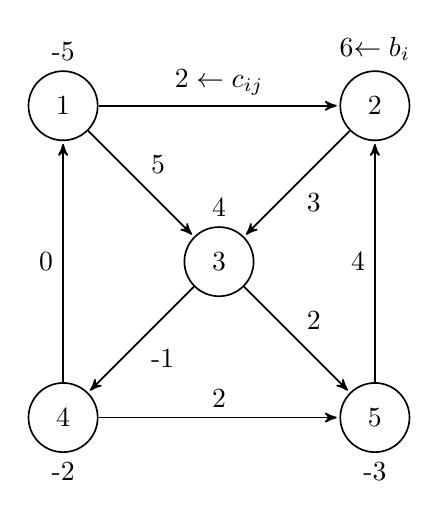
\begin{tikzpicture}[->,>=stealth',shorten >=1pt,auto,node distance=2.8cm,
                    semithick]

  \node[state] (node3) [label=above:4] {3};
  \node[state] (node1) [above left of=node3, label=above:-5] {1};
  \node[state] (node2) [above right of=node3, label=above:6$\leftarrow b_i$] {2};
  \node[state] (node4) [below left of=node3, label=below:-2] {4};
  \node[state] (node5) [below right of=node3, label=below:-3] {5};

  \path (node1) edge node {$2\leftarrow c_{ij}$} (node2)
        (node1) edge node {5} (node3)
        (node2) edge node {3} (node3)
        (node3) edge node {2} (node5)
        (node3) edge node {-1} (node4)
        (node4) edge node {0} (node1)
        (node4) edge node {2} (node5)
        (node5) edge node {4} (node2)
        ;
\end{tikzpicture}
\end{center}
You can also put them in figures like Figures \ref{fig:network2}--\ref{fig:network4}.
You can also draw a network that is slightly more graphical as in Figure \ref{fig:some_network}.
You can even draw a digram that is as complicated as Figure \ref{fig:complicated}.
Visit \url{http://www.texample.net/tikz/examples/} for more examples and ideas.








\begin{figure}
\begin{center}
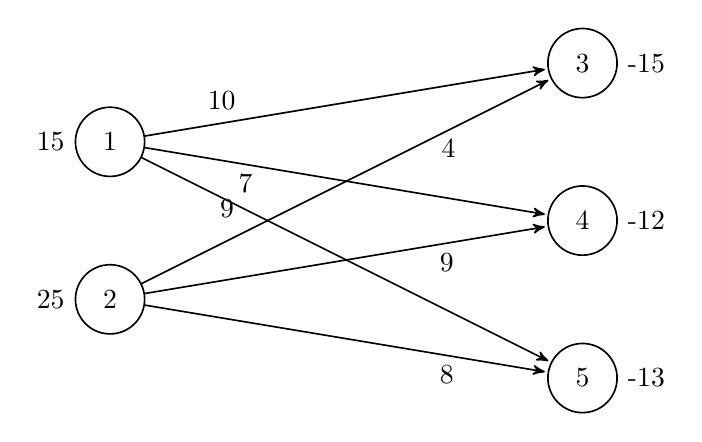
\begin{tikzpicture}[->,>=stealth',shorten >=1pt,auto,node distance=2.8cm,
                    semithick]

  \node[state] at(1,5) (node1) [label=left:15] {1};
  \node[state] at(1,3) (node2) [label=left:25] {2};
  \node[state] at(7,6) (node3) [label=right:-15] {3};
  \node[state] at(7,4) (node4) [label=right:-12] {4};
  \node[state] at(7,2) (node5) [label=right:-13] {5};

  \path (node1) edge node [near start]{10} (node3)
        (node1) edge node [near start, below]{7} (node4)
        (node1) edge node [near start, left]{9} (node5)
        (node2) edge node [near end, below]{4} (node3)
        (node2) edge node [near end, below]{9} (node4)
        (node2) edge node [near end, below]{8} (node5)
        ;

\end{tikzpicture}
\end{center}
\caption{Some network 2}
\label{fig:network2}
\end{figure}


\begin{figure}
\begin{center}
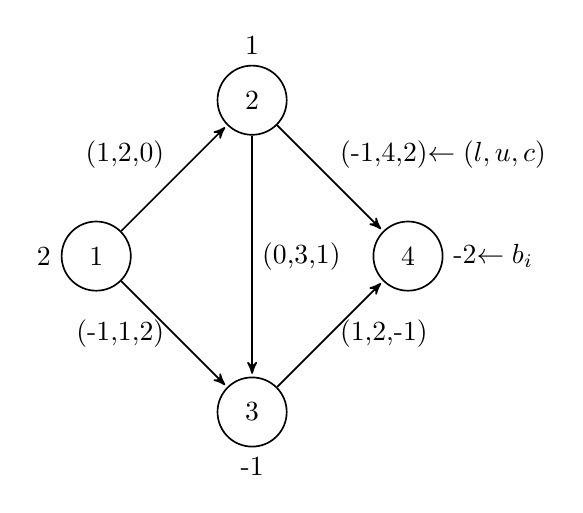
\begin{tikzpicture}[->,>=stealth',shorten >=1pt,auto,node distance=2.8cm,
                    semithick]

  \node[state] (node1) [label=left:2] {1};
  \node[state] (node2) [above right of=node1, label=above:1] {2};
  \node[state] (node3) [below right of=node1, label=below:-1] {3};
  \node[state] (node4) [below right of=node2, label=right:-2$\leftarrow b_i$] {4};

  \path (node1) edge node {(1,2,0)} (node2)
  		(node1) edge node [left] {(-1,1,2)} (node3)
  		(node2) edge node {(0,3,1)} (node3)
  		(node2) edge node {(-1,4,2)$\leftarrow(l,u,c)$} (node4)
  		(node3) edge node [right] {(1,2,-1)} (node4)
        ;
\end{tikzpicture}
\end{center}
\caption{Some network 3}
\label{fig:network3}
\end{figure}





\begin{figure}
	\centering
	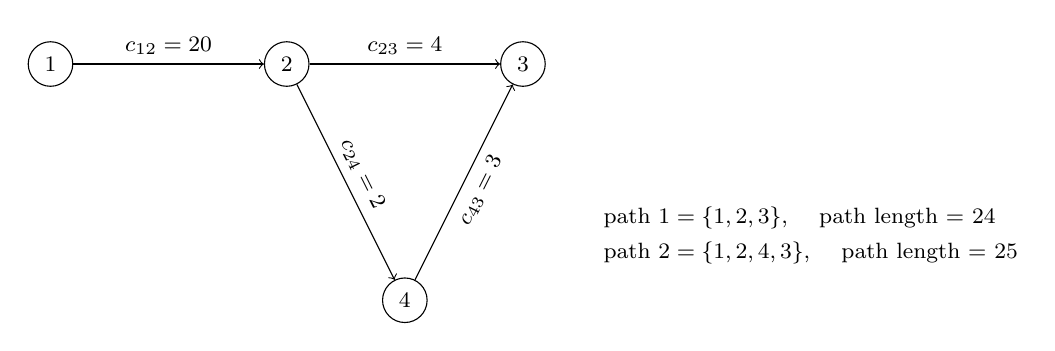
\begin{tikzpicture}[scale=0.3,auto,sloped]
	\tikzstyle{every node}=[font=\footnotesize]
	\node[shape=circle,draw] (n1) at (0,0) {1};
	\node[shape=circle,draw] (n2) at (10,0) {2};
	\node[shape=circle,draw] (n3) at (20,0) {3};
	\node[shape=circle,draw] (n4) at (15,-10) {4};
	
	\draw[->]
	(n1) edge node[above] {$c_{12}=20$} (n2)
	(n2) edge node[above] {$c_{23}=4$} (n3)
	(n2) edge node[above] {$c_{24}=2$} (n4)
	(n4) edge node[below] {$c_{43}=3$}  (n3)
	;
	
	\node[right] at (23,-6.5) {$\text{path } 1 = \{1,2,3\}$, \quad\text{path length} = 24};
	\node[right] at (23,-8)   {$\text{path } 2 = \{1,2,4,3\}$, \quad\text{path length} = 25};
	\end{tikzpicture}
	\caption{Some network 4}
	\label{fig:network4}
\end{figure}






\begin{figure} \centering
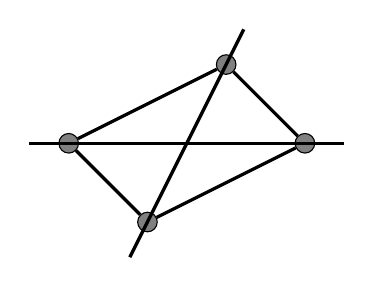
\begin{tikzpicture}[scale=1]
\tikzset{
    extended line/.style={
        to path={
            ($(\tikztostart)!-#1!(\tikztotarget)$) --  ($(\tikztotarget)!-#1!(\tikztostart)$) \tikztonodes
        }
    }
}
\tikzstyle{every node}=[circle, draw, fill=black!50,
                        inner sep=2.5pt, minimum width=4pt]

\node (n1) at (2,3) {};
\node (n2) at (3,5) {};
\node (n3) at (1,4) {};
\node (n4) at (4,4) {};

\draw [very thick] (n1) to[extended line=0.5cm] (n2);
\draw [very thick] (n3) to[extended line=0.5cm] (n4);
\draw [very thick] (n1) -- (n3);
\draw [very thick] (n2) -- (n4);
\draw [very thick] (n1) -- (n4);
\draw [very thick] (n2) -- (n3);
\end{tikzpicture}
\caption{Some network}
\label{fig:some_network}
\end{figure}














\begin{figure}\centering
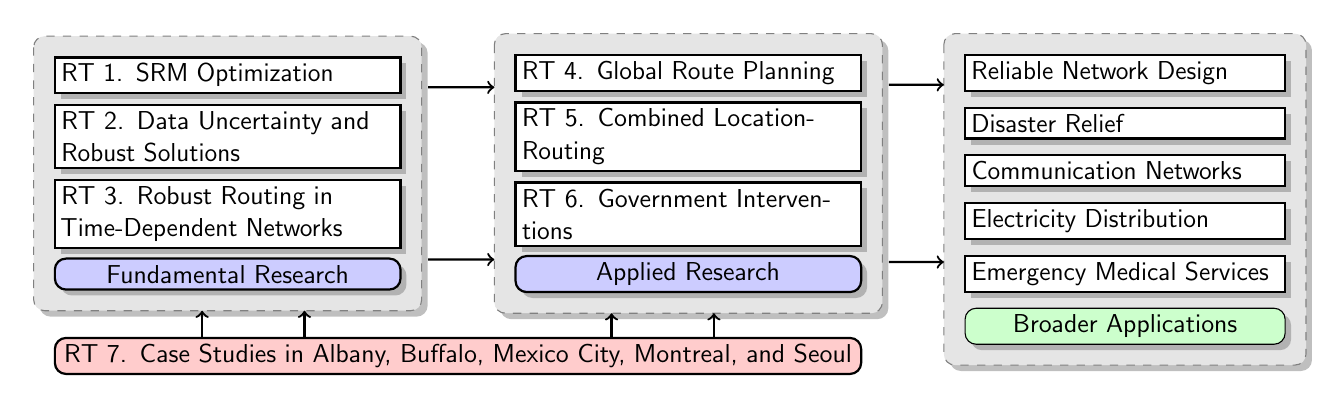
\begin{tikzpicture}[scale=0.65, transform shape, font=\Large\sffamily]

\tikzstyle{masterbox} = [inner sep=0]
\tikzstyle{bigbox} = [drop shadow, black, fill=gray!20!white,draw,inner sep=3.6pt, inner sep=7.5pt]
\tikzstyle{taskbox} = [drop shadow, thick, black, fill=white,draw, text width=6.5cm, inner sep=3.6pt]
\tikzstyle{researchbox} = [drop shadow, thick, black, fill=blue!20!white,draw,rounded corners, text width=6.5cm, text centered, inner sep=3.6pt]
\tikzstyle{babox} = [drop shadow, thick, black, fill=white,draw, text width=6cm, inner sep=3.6pt]
\tikzstyle{broaderbox} = [drop shadow, black, fill=green!20!white,draw,rounded corners, text width=6cm, text centered, inner sep=3.6pt]
\tikzstyle{casebox} = [thick, black, fill=red!20!white,draw,rounded corners, text width=15.5cm, text centered,inner sep=3.6pt]

\node[casebox] (case) {
	RT 7. Case Studies in Albany, Buffalo, Mexico City, Montreal, and Seoul
};

\node[researchbox, above=1.6cm of case.west, anchor=west] (fr) {Fundamental Research};
\node[taskbox, above=3.2cm of fr] (rt1) {RT 1. SRM Optimization};
\node[taskbox, below=0.2cm of rt1] (rt2) {RT 2. Data Uncertainty and Robust Solutions};
\node[taskbox, below=0.2cm of rt2] (rt3) {RT 3. Robust Routing in Time-Dependent Networks};

\begin{pgfonlayer}{background}
	\path (rt1.west |- rt1.north)+(-0.4,0.4) node (box1a) {};
	\path (fr.east |- fr.south)+(0.4,-0.4) node (box1b) {};
	\path [fill=black!10, drop shadow, rounded corners, draw=black!50, dashed] (box1a) rectangle (box1b);
\end{pgfonlayer}

\node[researchbox, above=1.6cm of case.east, anchor=east] (er) {Applied Research};
\node[taskbox, above=3.2cm of er] (rt4) {RT 4. Global Route Planning};
\node[taskbox, below=0.2cm of rt4] (rt5) {RT 5. Combined Location-Routing};
\node[taskbox, below=0.2cm of rt5] (rt6) {RT 6. Government Interventions};

\begin{pgfonlayer}{background}
	\path (rt4.west |- rt4.north)+(-0.4,0.4) node (box2a) {};
	\path (er.east |- er.south)+(0.4,-0.4) node (box2b) {};
	\path [fill=black!10, drop shadow, rounded corners, draw=black!50, dashed] (box2a) rectangle (box2b);
\end{pgfonlayer}

\path (box1a -| box1b) + (0,-1cm) node (box1c) {};
\path (box1b) + (0,1cm) node (box1d) {};
\draw[->,thick] (box1c) -- (box1c -| box2a);
\draw[->,thick] (box1d) -- (box1d -| box2a) ;


\node[babox, right=2cm of rt4] (ba1) {Reliable Network Design};
\node[babox, below=0.3cm of ba1] (ba2) {Disaster Relief};
\node[babox, below=0.3cm of ba2] (ba3) {Communication Networks};
\node[babox, below=0.3cm of ba3] (ba4) {Electricity Distribution};
\node[babox, below=0.3cm of ba4] (ba5) {Emergency Medical Services};
\node[broaderbox, below=0.3cm of ba5] (ba) {Broader Applications};

\begin{pgfonlayer}{background}
	\path (ba1.west |- ba1.north)+(-0.4,0.4) node (box3a) {};
	\path (ba.east |- ba.south)+(0.4,-0.4) node (box3b) {};
	\path [fill=black!10, drop shadow, rounded corners, draw=black!50, dashed] (box3a) rectangle (box3b);
\end{pgfonlayer}

\path (box2a -| box2b) + (0,-1cm) node (box2c) {};
\path (box2b) + (0,1cm) node (box2d) {};
\draw[->,thick] (box2c) -- (box2c -| box3a);
\draw[->,thick] (box2d) -- (box2d -| box3a) ;



\draw[->,thick] ([xshift=-5cm]case.north) -- ([xshift=-5cm]case.north |- box1b);
\draw[->,thick] ([xshift=-3cm]case.north) -- ([xshift=-3cm]case.north |- box1b);

\draw[->,thick] ([xshift=5cm]case.north) -- ([xshift=5cm]case.north |- box2b);
\draw[->,thick] ([xshift=3cm]case.north) -- ([xshift=3cm]case.north |- box2b);

\end{tikzpicture}
\caption{Complicated diagram}
\label{fig:complicated}
\end{figure}



\end{document}







%
